\documentclass{beamer}
\usetheme[hideothersubsections]{HRTheme}
\usepackage{beamerthemeHRTheme}
\usepackage{graphicx}
\usepackage[space]{grffile}
\usepackage{listings}
%\usepackage{animate}
\lstset{language=SQL,
basicstyle=\ttfamily\footnotesize,
mathescape=true,
keywordstyle=\color{blue},
breaklines=true,
showspaces=false,
showstringspaces=false}
\usepackage[utf8]{inputenc}
\usepackage{color}
\newcommand{\red}[1]{
\textcolor{red}{#1}
}
\newcommand{\ts}{\textbackslash}


\title{Document Database and MapReduce}
\author{ }
\institute{Hogeschool Rotterdam \\ 
Rotterdam, Netherlands}

\date{}

\begin{document}
\maketitle

\SlideSection{Introduction}
\SlideSubSection{Lecture topics}
\begin{slide}{
\item CAP Theorem ACID vs BASE
\item Document Databases 
\item MongoDB
\item Map-Reduce 
\item Summery
}\end{slide}

\SlideSection{NoSQL database and CAP theorem}
\SlideSubSection{Motivation}
\begin{slide}{
\item As we mentioned before relational database systems are designed to run on a single server
\item RDBMS satisfy the ACID rules to provide consistency and availability of the data for the users  
\item But how do NoSQL databases deal with the data in their implementation?
}\end{slide}

\SlideSection{NoSQL database and CAP theorem}
\SlideSubSection{CAP theorem}
\begin{slide}{
\item States that it is impossible for a distributed computer system to simultaneously provide all three of the following guarantees:
\begin{itemize}
	\item \textbf{Consistency} every read receives the most recent write or an error
	\item \textbf{Availability} every request receives a response, without guarantee that it contains the most recent version of the information
	\item \textbf{Partition} tolerance (the system continues to operate despite arbitrary partitioning due to network failures
\end{itemize}
}\end{slide}


\SlideSection{NoSQL database and CAP theorem}
\SlideSubSection{ACID vs BASE}
\begin{slide}{
\item \textbf{B}asically \textbf{A}vailable, \textbf{S}oft State
and  Eventual \textbf{C}onsistent \\
\item Because of this characteristic the query language must be able to process data saved locally and in a cluster (to be discussed in another slide)  
\begin{figure}
		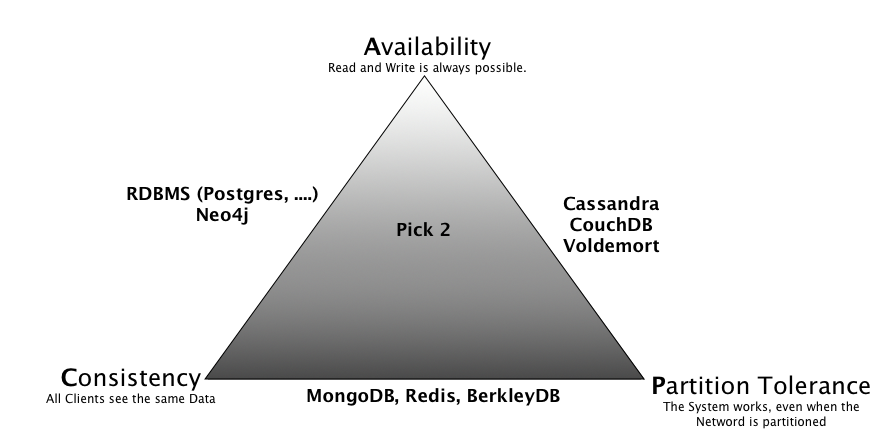
\includegraphics[scale=0.25]{img/cap}
		\caption{CAP Theorem}
\end{figure}
}\end{slide}

\SlideSection{RDBMS vs Document database}
\begin{slide}{
\item Relational databases are considered to be structural
\item Document databases uses semi-structured formats 
\item text files such as logs are unstructured
}\end{slide}


\SlideSection{Document Database}
\SlideSubSection{Introduction}
\begin{slide}{
\item A document database is a nonrelational database that stores data as semi-structured documents such as in XML or JSON formats
\item Document databases are free to implement ACID transactions or other characteristics of a traditional RDBMS
\item A document database allows some form of data description without enforcing a schema
\item The alignment with web-development programming practices has resulted in JSON and document databases/storage
}\end{slide}	

\SlideSubSection{Introduction}
\begin{slide}{
\item Let us see what are those formats and how they are used!
\item We will start with eXtensible Markup Language 
\item Then we will look at JavaScript Object Notation and it's Binary version 
}\end{slide}

\SlideSubSection{eXtensible Markup Language (XML)}
\begin{slide}{
\item Defined by the WWW Consortium (W3C)
\item Extensible, unlike HTML, users can add new tags, and separately specify how the tag should be handled for display	 
\item XML has become the basis for all new generation data interchange formats. For instance bank transfers and secure document exchange
\item Documents have tags giving extra information about sections of the document. Those tags can also be nested
}\end{slide}

\begin{frame}[fragile]{HTML as XML }
\begin{lstlisting}
<!DOCTYPE html>
<html xmlns="http://www.w3.org/1999/xhtml">
  <head>
    <meta charset="UTF-8"/>
    <title>Polyglot (X)HTML Template</title>
  </head>
  <body>
    <p>content....</p>
  </body>
</html>
\end{lstlisting}
\end{frame}

\SlideSubSection{XML}
\begin{slide}{
\item Each XML based standard defines what are valid elements, using XML type specification languages to specify the syntax
\item DTD (Document Type Descriptors): describes the structure of an XML document
\item XML Schema (newer than DTD): a special type of XML document that describes the elements that may be present
\item Sample implementation database BaseX (basex.org)
}\end{slide}

\begin{frame}[fragile]{Document Type Descriptors}
\begin{lstlisting}
<! ELEMENT department(dept_name, building, budget)>
<! ELEMENT dept_name (#PCDATA)>
<! ELEMENT budget (#PCDATA)>
<! ELEMENT university ( ( department | course | instructor | teaches )+)>


Notation:
	|	: alternatives
	+	:  1 or more occurrences
	* 	:  0 or more occurrences
	#PCDATA	:	Parsed charachter data i.e. parsed string
\end{lstlisting}
\end{frame}



\SlideSubSection{XML Processing}
\begin{slide}{
\item XPath: A syntax for retrieving specific elements from an XML document using wildcards.
\item XQuery: A query language provides mechanisms for modifying a document. XQuery is sometimes referred to as “the SQL of XML".
\item  XSLT (Extensible Stylesheet Language Transformations): A language for transforming XML documents into alternative formats, including non-XML formats such as HTML.
\item DOM (Document Object Model): An object-oriented API that programs can use to interact with XML, XHTML, and similarly structured documents.
}\end{slide}

\SlideSubSection{Tree Model of XML Data}
\begin{slide}{
\item Query and transformation languages are based on a tree model of XML data
\item An XML document is modeled as a tree, with nodes corresponding to elements and attributes
\begin{figure}
		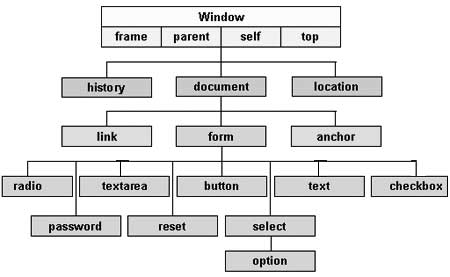
\includegraphics[scale=0.3]{img/html-dom}
		\caption{DOM sample of an HTML document}
\end{figure}
}\end{slide}


\SlideSubSection{XML Processing: XPath}
\begin{slide}{
\item XPath: is used to address (select) parts of documents using path expressions
\begin{itemize}
\item  The initial denotes root of the document (above the top-level tag) 
\item Think of file names in a directory hierarchy
\item Selection predicates may follow any step in a path, in [ ] 
\item It is possible to apply selection criteria on the values using comparison operators \footnote{ \href{http://www.w3schools.com/xsl/xpath_examples.asp}{Demonstrate an  example}}
\end{itemize}
}\end{slide}


\SlideSubSection{XML Processing: XQuery and XPath}
\begin{slide}{
\item XQuery is derived from the Quilt query language, which itself borrows from SQL.
\item XQuery uses a:    for … let … where … order by …result …  \footnote{  \textbf{let}: allows temporary variables, and has no equivalent in SQL}
\footnote{ \href{http://www.w3schools.com/xsl/xquery_flwor.asp}{Demonstrate an example}}
\begin{itemize}
	\item for			=	 from 
	\item where		=	 where
	\item order by	=	 order by
	\item result		=	 select
\end{itemize}
}\end{slide}

\SlideSubSection{JavaScript Object Notation JSON}
\begin{slide}{
\item JSON is an open-standard format that uses human-readable text to transmit data objects consisting of attribute–value pairs
\item JSON Schema is based on the concepts from XML Schema, but is JSON-based
\item Document databases use JSON documents in order to store records, just as tables and rows store records in a relational database
}\end{slide}

\SlideSubSection{BSON}
\begin{slide}{
\item BSON: binary-encoded format used in MongoDB instead of JSON
\item BSON extends the JSON model to provide additional data types such as integer and float to be efficient for encoding and decoding within different languages.
\item BSON implementation supports embedding objects and arrays within other objects and arrays
}\end{slide}


\SlideSubSection{MongoDB}
\begin{slide}{
\item A MongoDB instance may have zero or more databases
\item A database may have zero or more collections.
\begin{itemize}
	\item Can be thought of as the relation (table) in DBMS, but with many differences.
\end{itemize}
\item A collection may have zero or more documents.
\pause
\begin{itemize}
	\item Docs in the same collection don’t even need to have the same
fields
	\item Docs are the records in RDBMS
	\item Docs can embed other documents
	\item Documents are addressed in the database via a unique key differences.
\end{itemize}
\pause
\item A document may have one or more fields.
\item query language is JavaScript
\item Threre is no join provided in MongoDB. You have to implement it manually.
}\end{slide}



\SlideSection{Document Data-Model}
\SlideSubSection{Relational Model}
\begin{slide}{
\item Suppose you have the following entities and their relationships
\begin{figure}
		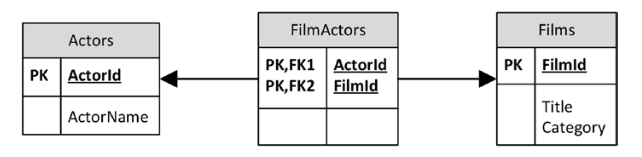
\includegraphics[scale=0.3]{img/mongo-relational}
\end{figure}
\item How would we model this in a document structure?
}\end{slide}


\SlideSubSection{Embedded}
\begin{slide}{
	\item First mapping possibility is to map to one embedded collection.
\begin{figure}
		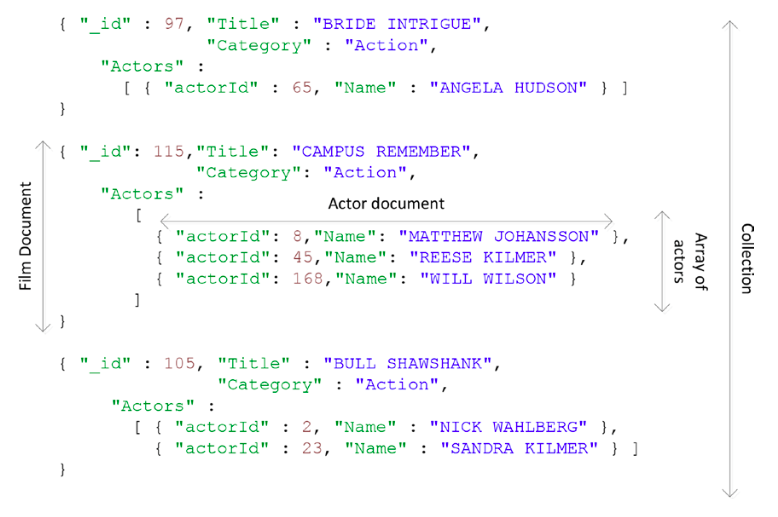
\includegraphics[scale=0.23]{img/mongo-embeded}
\end{figure}
 \item document database are not designed to be normalized and data repetition is accepted, but could have side effects.   
}\end{slide}


\SlideSubSection{Linking using object \textunderscore id}
\begin{slide}{
	\item Second mapping possibility is to map to different collections and link the documents
\begin{figure}
		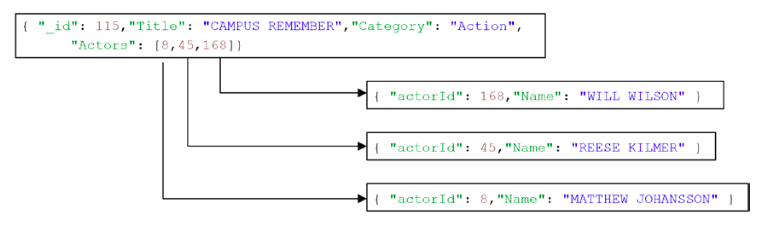
\includegraphics[scale=0.3]{img/mongo-linked}
\end{figure}
\item This approach is less suited for document databases since the binary data of those collections are not stored as a continuous stream.
\item Another disadvantage of this approach is the lack of join query
}\end{slide}



\begin{frame}[fragile]{Querying collections and objects}
\begin{itemize}
\item Select queries in MongoDB 
\end{itemize}
\begin{lstlisting}
\\SQL
SELECT * FROM actors

SELECT * FROM actors WHERE age = 23 

SELECT * FROM actors WHERE age = 23 ORDER BY name

\\Mongo
db.actors.find()

db.actors.find({age: 23})

db.actors.find({age: 23}).sort({name:1})
\end{lstlisting}
\end{frame}


\begin{frame}[fragile]{Querying collections and objects}
\begin{itemize}
\item Insert queries in MongoDB 
\item Suppose we have a relationship between actor entity and address entity based on actor\textunderscore id
\end{itemize}
\begin{lstlisting}
\\SQL
INSERT INTO actors(actor_id,name,age) 
	VALUES(3, "actor name", 45)
INSERT INTO address(addressid, street, city, actor_id) 
	VALUES(5, "Wijnhaven 66", "Rotterdam", 3)

\\Mongo
db.actors.insert({name:"actor name", age: 23, 
		address:{street:"Wijnhaven 66", city:"Rotterdam"}
	})
\end{lstlisting}
\end{frame}

\begin{frame}[fragile]{Querying collections and objects}
\begin{itemize}
\item Update queries in MongoDB 
\end{itemize}
\begin{lstlisting}
\\SQL
UPDATE actors
	SET name = "New name" 
	WHERE actor_id = "a1"

\\Mongo
db.actors.update(
   { _id: "a1" },
 \\& sould be dollar
   { &set : {
   		name: "New Name"} 
   	})
\end{lstlisting}
\end{frame}


\SlideSection{MapReduce}
\SlideSubSection{Introduction}
\begin{slide}{
\item MapReduce is a data processing paradigm for condensing large volumes of data into useful aggregated results.
\item Map- and Reduce functions are commonly used in functional programming   
\item In INFDEV02-2 and INDEV02-3 we already introduced HOFs
\item MapReduce rely on the concept of higher order functions HOFs are very powerful in the context of NoSQL databases. 
\item The following functions will be further discussed : FlatMap, Map and Reduce 
}\end{slide}


\begin{frame}[fragile]{Map Function}
\begin{itemize}
\item Apply the function f to each element of list x
\item map(f, x[0...n-1])
\item in Python: \\
\end{itemize}
\begin{lstlisting}
def square(x):  
	return x * x 

map(square, [1, 2, 3, 4])  #would return [1, 4, 9, 16]
 \end{lstlisting}
\begin{figure}
		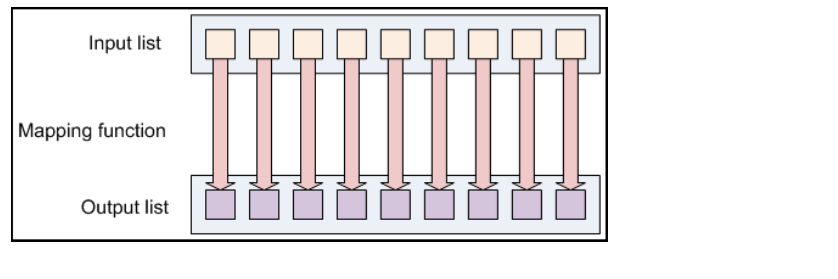
\includegraphics[scale=0.23]{img/map}
\end{figure}
\end{frame}

\begin{frame}[fragile]{Reduce Function}
\begin{itemize}
\item Repeatedly apply binary function f to pairs of items in x, replacing the pair of items with the result until only one item remains
\item reduce(f, x[0...n-1])
\item in Python: \\
\end{itemize}
\begin{lstlisting}
def add(x,y): 
	return x+y 
reduce(add, [1,2,3,4]) #would result in a 10
\end{lstlisting}
\begin{figure}
		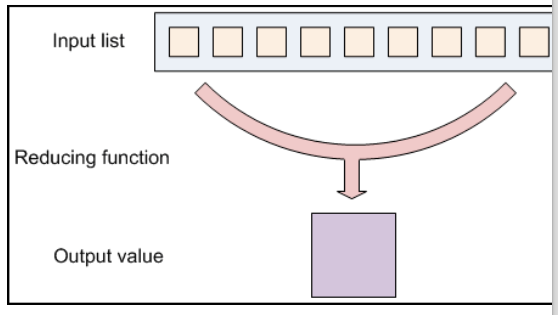
\includegraphics[scale=0.23]{img/reduce}
\end{figure}
\end{frame}

\begin{frame}[fragile]{FlatMap Function}
\begin{itemize}
\item Repeatedly apply function f to items in a sublist, then removing the sublist structure with the result of one dimensional list
\item FlatMap(f, x[[0..n-1],[0..m-1]])
\item in pseudo Python: suppose the f function returns the element without any change\\
\end{itemize}
\begin{lstlisting}
listOfLists = [[1, 2],[3, 4, 5], [6]]
for l in  listOfLists:
	map(f, l)
reduce(list.__add__, listOfLists)
#would result in a flatten list [1, 2, 3, 4, 5, 6]
\end{lstlisting}
\end{frame}

\SlideSubSection{SQL and MapReduce}
\begin{slide}{
\item We have seen so far what map en reduce functions are
\item But why do we need them in document sturcture?
\item What are the similarities between MapReduce and SQL?
}\end{slide}

\SlideSubSection{MapReduce Function in MongoDB}
\begin{slide}{
\item Data in mongoDB are saved in documents
\item The MapReduce function first queries the collection, then maps the result documents to emit key-value pairs which is then reduced based on the keys that have multiple values.
\begin{figure}
		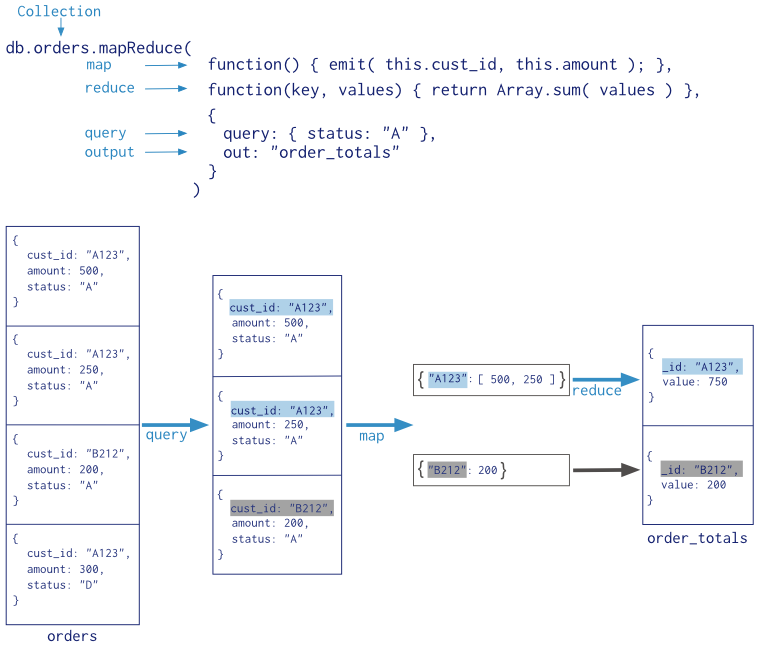
\includegraphics[scale=0.26]{img/map-reduce}
\end{figure}
}\end{slide}

\SlideSubSection{Map and Filter functions vs SQL}
\begin{slide}{
\item Relational databases use the map, filter and reduce paradigm (where it is called project, select, aggregate).
\item SELECT MAX(pixels) FROM  cameras WHERE brand = 'Nikon' 
\begin{itemize}
\item cameras is a sequence (a list of rows, where each row has the data for one camera)
\item WHERE brand = 'Nikon'  is a \textbf{filter}
\item pixels is a \textbf{map} (extracting just the pixels field from the row)
\item MAX is a \textbf{reduce}
\end{itemize}
\item Demo!
}\end{slide}

\SlideSubSection{Join as MapReduce in MongoDB}
\begin{slide}{
\item MongoDb does not provide explicit join queries to join two collections
\item To implement a join you need 
\begin{itemize}
\item  a mapper for each collection to retrieve key and values for each collection 
\item A reducer function to reduce values for each key
\end{itemize}
\item Demo! 
}\end{slide}

\SlideSubSection{MapReduce Function in a Cluster}
\begin{slide}{
\item How does CAP theorem effect the implementation of MapReduce?
\item Generally speaking It depends on the execution of MapReduce whether local or in a cluster 
\item We have seen how MapReduce is executed locally in document database 
\item What about clusters?
}\end{slide}

\SlideSubSection{MapReduce Function in a Cluster}
\begin{slide}{
\item The distributed MapReduce idea is similar to (but not the same as!): reduce(f2, map(f1, x))
\item Key idea: "data-centric" architecture –  Send function f1 directly to the data : Execute it concurrently
\item Then merge results with reduce: Also concurrently
}\end{slide}

\SlideSubSection{End}
\begin{slide}{
\item Thank you and the best of luck!
}\end{slide}

\end{document}

\begin{slide}{
\item ...
}\end{slide}

\begin{frame}[fragile]
\begin{lstlisting}
...
\end{lstlisting}
\end{frame}
